\documentclass[a4paper,11pt]{article}\usepackage[]{graphicx}\usepackage[]{color}
%% maxwidth is the original width if it is less than linewidth
%% otherwise use linewidth (to make sure the graphics do not exceed the margin)
\makeatletter
\def\maxwidth{ %
  \ifdim\Gin@nat@width>\linewidth
    \linewidth
  \else
    \Gin@nat@width
  \fi
}
\makeatother

\definecolor{fgcolor}{rgb}{0.345, 0.345, 0.345}
\newcommand{\hlnum}[1]{\textcolor[rgb]{0.686,0.059,0.569}{#1}}%
\newcommand{\hlstr}[1]{\textcolor[rgb]{0.192,0.494,0.8}{#1}}%
\newcommand{\hlcom}[1]{\textcolor[rgb]{0.678,0.584,0.686}{\textit{#1}}}%
\newcommand{\hlopt}[1]{\textcolor[rgb]{0,0,0}{#1}}%
\newcommand{\hlstd}[1]{\textcolor[rgb]{0.345,0.345,0.345}{#1}}%
\newcommand{\hlkwa}[1]{\textcolor[rgb]{0.161,0.373,0.58}{\textbf{#1}}}%
\newcommand{\hlkwb}[1]{\textcolor[rgb]{0.69,0.353,0.396}{#1}}%
\newcommand{\hlkwc}[1]{\textcolor[rgb]{0.333,0.667,0.333}{#1}}%
\newcommand{\hlkwd}[1]{\textcolor[rgb]{0.737,0.353,0.396}{\textbf{#1}}}%
\let\hlipl\hlkwb

\usepackage{framed}
\makeatletter
\newenvironment{kframe}{%
 \def\at@end@of@kframe{}%
 \ifinner\ifhmode%
  \def\at@end@of@kframe{\end{minipage}}%
  \begin{minipage}{\columnwidth}%
 \fi\fi%
 \def\FrameCommand##1{\hskip\@totalleftmargin \hskip-\fboxsep
 \colorbox{shadecolor}{##1}\hskip-\fboxsep
     % There is no \\@totalrightmargin, so:
     \hskip-\linewidth \hskip-\@totalleftmargin \hskip\columnwidth}%
 \MakeFramed {\advance\hsize-\width
   \@totalleftmargin\z@ \linewidth\hsize
   \@setminipage}}%
 {\par\unskip\endMakeFramed%
 \at@end@of@kframe}
\makeatother

\definecolor{shadecolor}{rgb}{.97, .97, .97}
\definecolor{messagecolor}{rgb}{0, 0, 0}
\definecolor{warningcolor}{rgb}{1, 0, 1}
\definecolor{errorcolor}{rgb}{1, 0, 0}
\newenvironment{knitrout}{}{} % an empty environment to be redefined in TeX

\usepackage{alltt}
\usepackage{graphicx,fancyhdr}
\newcommand{\rinline}[1]{SOMETHING WRONG WITH knitr}
\usepackage{amsmath,amssymb}
\usepackage[british]{babel}
\usepackage{natbib}
\usepackage{booktabs}
\newcommand{\iid}{\stackrel{\mathrm{iid}}{\sim}}
\oddsidemargin  0in
\evensidemargin  0in
\textwidth   6.3in
\textheight  9.5in
\topmargin  -0.7in
\renewcommand{\baselinestretch}{1.2}

%\input{macros.tex}
\def\CO{{CO$_{2}$}}
\IfFileExists{upquote.sty}{\usepackage{upquote}}{}
\begin{document}
%\SweaveOpts{concordance=TRUE}
\thispagestyle{empty}
\title{Analysis of \CO\ data at Mauna Loa}
\author{
A.~C.~Davison\footnote{Institute of Mathematics, IMA-FSB-EPFL, Station 8, 
Ecole Polytechnique F\'ed\'erale de Lausanne,
1015 Lausanne, Switzerland, {\tt Anthony.Davison@epfl.ch}} 
} 
\date{\today}

\maketitle 
{
\bigskip\centerline{\bf Summary\footnote{Summary: a short summary of the report, with approximately one sentence for each section.  Should not contain formulae}  }

\noindent This report\footnote{Use of footnotes should be avoided in scientific writing: if something is important enough to be included, it should be in the text.  However in this document footnotes are used to highlight a few presentational points.}   describes a time series analysis of the \CO\ data from the Mauna Loa observatory, the so-called Keeling curve, which was one of the earliest measured signs of the effect of human activity on the global environment.  The data show strong slightly super-linear trend and seasonality, rising over the period 1958--2008 from 315--385ppmv, and marked annual variation of around 5ppmv.  A seasonal ARIMA model fits the data well.  Predictions from it suggest that the level 400ppmv will be breached in around 2015, or perhaps slightly earlier.
 }

\newpage

%%%%%%%%%%%%%%%%%%%%%%%%%%%
% set options for LaTeX and Sweave

\setkeys{Gin}{width=\textwidth} 
%%%%%%%%%%%%%%%%%%%%%%%%%%%

%%%%%%%%%%%%%%%%%%%%%%%%%%%
\section{Initial data analysis}

The data\footnote{Introductory section:   presentation of the data; exploratory data analysis (trend,  
seasonality, correlograms, periodograms); purpose of the analysis.}  we consider are monthly mean atmospheric carbon dioxide at Mauna Loa Observatory, Hawaii.  These data, measured as the dry mole fraction---defined as the number of molecules of carbon dioxide divided by the number of molecules of dry air---and given in units of parts per million by volume  (ppmv), constitute the longest record of direct observation of \CO\  in the atmosphere. Measurements were started in March of 1958 and are currently available to the end of November 2008.  A graph of the data, the so-called Keeling curve, is considered as iconic in climate change, as it was one of the earliest indications of the effect of human activities on the global climate.  The data may be downloaded from a link from the page
\begin{verbatim}
http://www.esrl.noaa.gov/gmd/ccgg/trends/co2_data_mlo.html
\end{verbatim}
where further details may be found; see also the Wikipedia article on the `Keeling curve' and the Scripps Institute of Oceanography website, \begin{verbatim}
http://scrippsco2.ucsd.edu/
\end{verbatim}
In this report we analyse these observations with a view towards prediction of the values to the year 2020.

%%%%%%%%%%%%%%%%%%%%%%%%%%%

%%%%%%%%%%%%%%%%%%%%%%%%%%%

Figure~\ref{data.fig} shows the data.\footnote{The caption for the figure should give the units of measurement and enough detail for the figure to be read without reference to the text. Both axes should be labelled.  However, interpretation of the plot is left to the text.}  The two most striking features are the strong upward trend, as the \CO\  level rises from around 315ppmv to around 385ppmv over the 50 years, and the pronounced seasonal pattern.  The trend is essentially piecewise linear, but apparently slightly convex, suggested a possible acceleration of the trend over the period of the data, and particularly perhaps from the late 1990s.  The seasonality accounts for variation of around 5ppmv, and seems to vary slightly from year to year. 

\begin{figure}[h]
\begin{center}
%%%%%%%%%%%%%%%%%%%%%%%%%%%
\begin{knitrout}
\definecolor{shadecolor}{rgb}{0.969, 0.969, 0.969}\color{fgcolor}
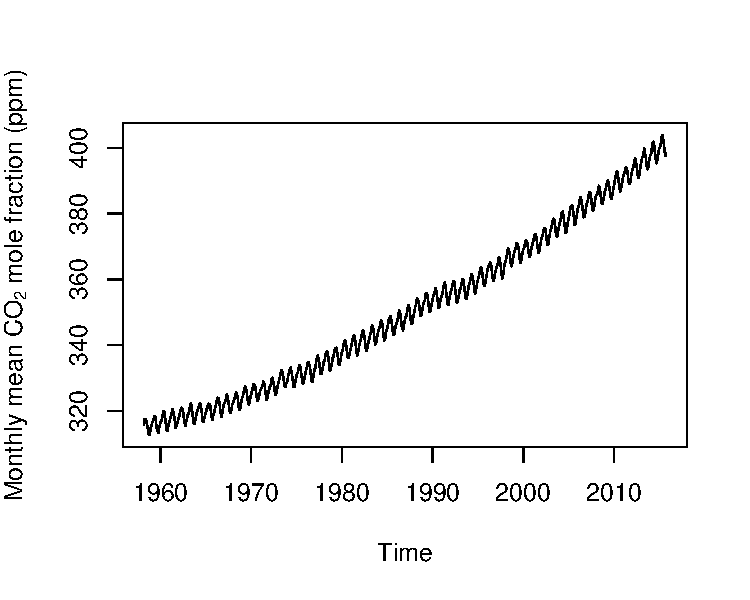
\includegraphics[width=\maxwidth]{figure/CO2-figinit-1} 

\end{knitrout}
%%%%%%%%%%%%%%%%%%%%%%%%%%%
\end{center}
\caption{Mean monthly atmospheric \CO\ (ppmv) at Mauna Loa, Hawaii, from March 1958 to November 2008.}
\label{data.fig}
\end{figure}

STL decomposition \citep{STL:1990}\footnote{Note the format for references.} of the data, shown in Figure~\ref{stl.fig}, confirms these remarks.  The seasonality is due to annual changes in vegetation in the northern hemisphere: the level of carbon dioxide in the atmosphere decreases from northern spring onwards as new plant growth takes the gas out of the atmosphere through photosynthesis, and rises again in the northern autumn when plants and leaves die off and decay to release the gas. When plotted with a different aspect ratio, the cycle is clearly non-sinusoidal, and appears to fluctuate somewhat in magnitude, broadly being smaller from 1960--1975 and around the year 2000 than in the 1990s and at present.  This variation is difficult to explain.  If it is not random fluctuation, it may indicate changes in the carbon cycle due to a gradual increase in global population on which is superimposed the destruction of rainforests, the collapse of heavy industry in Eastern Europe after 1990, and the more recent rapid industrialisation of China.  It might also be due partly to volcanic effects.  The trend in the STL plot shows more clearly a broad convex form, and the residuals show some positive autocorrelation. 

\begin{figure}[ht]
\begin{center}
%%%%%%%%%%%%%%%%%%%%%%%%%%%
\begin{knitrout}
\definecolor{shadecolor}{rgb}{0.969, 0.969, 0.969}\color{fgcolor}
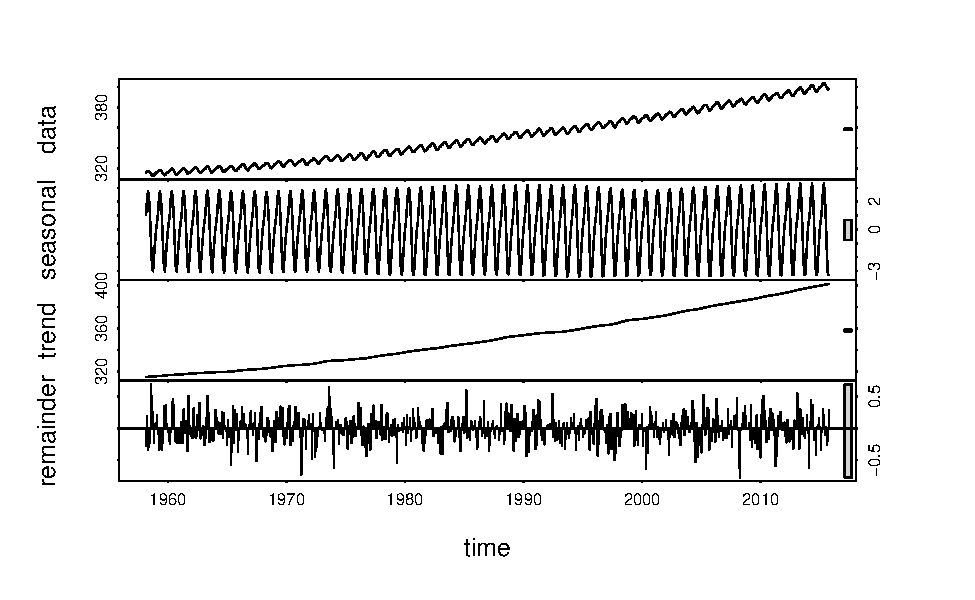
\includegraphics[width=\maxwidth]{figure/CO2-STLdecomp-1} 

\end{knitrout}
%%%%%%%%%%%%%%%%%%%%%%%%%%%
\end{center}
\caption{Mauna Loa data and its STL decomposition.  Top panel: data. Second panel: seasonal effect.  Third panel: trend.  Fourth panel: residuals.  The grey bar on the right is for comparison of the sizes of the different components. }
\label{stl.fig}
\end{figure}

Figure~\ref{spec.fig} shows the periodogram of the data, without and with three different degrees of smoothing.  The anticipated peak at one cycle/year stands out very clearly, as do other peaks at 2, 3, and perhaps 4 cycles/year, which are harmonics of the annual cycle.  There is also a peak on the left due to the overall trend, indistinguishable from very low-frequency variation, but apart from the harmonics and a dip at 3.5 cycles/year, the spectrum seems to be essentially flat from 2 cycles/year upwards.  

\begin{figure}[htbp]
\begin{center}
%%%%%%%%%%%%%%%%%%%%%%%%%%
\begin{knitrout}
\definecolor{shadecolor}{rgb}{0.969, 0.969, 0.969}\color{fgcolor}
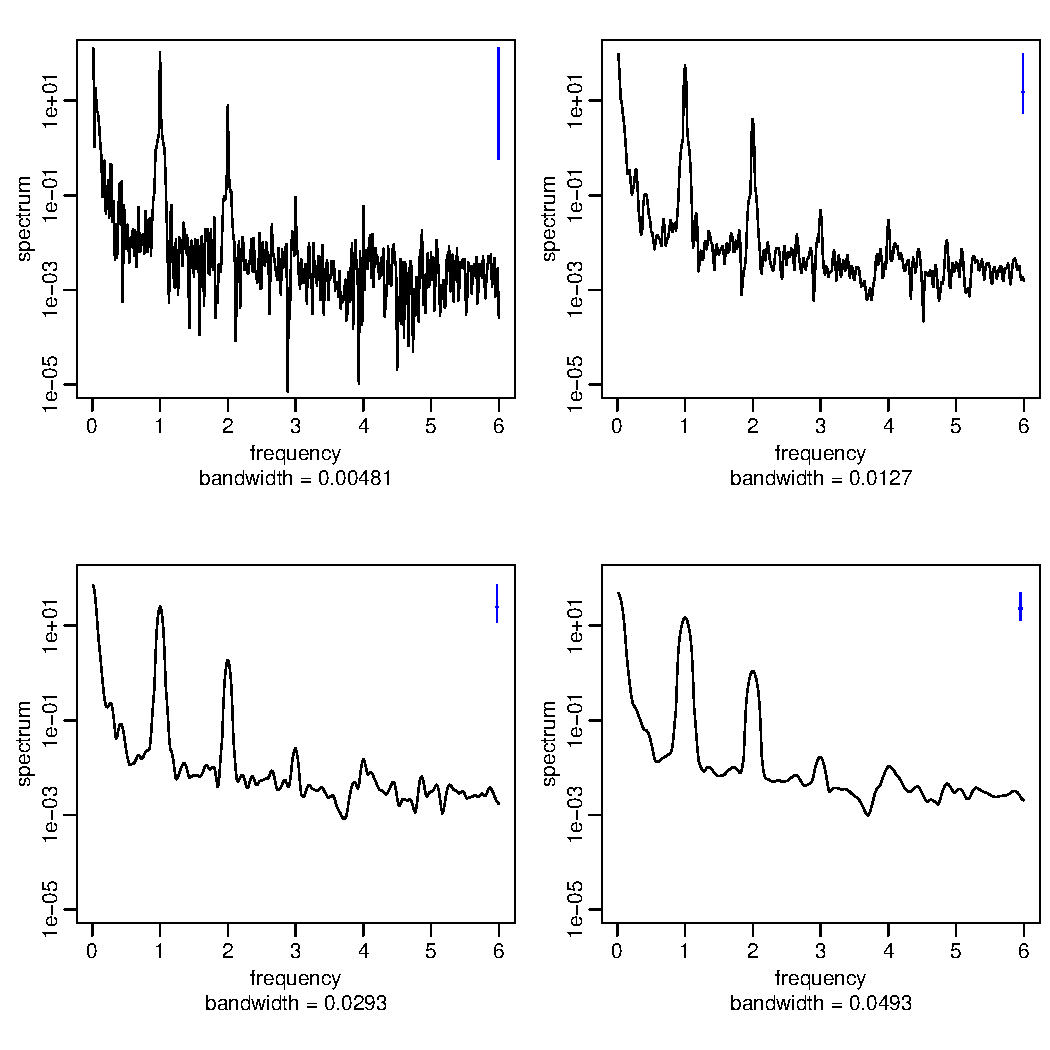
\includegraphics[width=\maxwidth]{figure/CO2-spectrum-1} 

\end{knitrout}
%%%%%%%%%%%%%%%%%%%%%%%%%%%
\end{center}
\caption{Frequency domain analysis of Mauna Loa data.  Top left: raw periodogram. The remaining panels show successively more smoothed periodograms, with the effective bandwidth given under each panel and shown as the center line of the calibration bar at the top right of each panel.  The height of the calibration bar shows significant variation in the periodogram.}
\label{spec.fig}
\end{figure}

With a view to the possible fitting of SARIMA models, Figure~\ref{diff.fig} shows the correlogram and partial correlogram of the data differenced at one lag to remove the trend and at 12 lags to remove the seasonal component, that is, of\footnote{Any displayed equations should be punctuated as parts of sentences.  Punctuation rules of English grammar should be used for a report written in English, and of French grammar for a report written in French.}
\begin{align}
\label{x.eqn}
x_t=(I-B)(I-B^{12})y_t,
\end{align}
where $\{y_t\}$ represents the original data and $B$ the backshift operator.  Of the two plots the correlogram  seems simpler: the strong negative correlation at lag 12, but not at lag 24, 36, $\ldots$, suggests a seasonal moving average component of order $Q=1$, and the significant correlations at lags $h=1, 11, 13$ suggest a moving average component of order $q=1$.  

\begin{figure}[ht!]
\begin{center}
%%%%%%%%%%%%%%%%%%%%%%%%%%%
\begin{knitrout}
\definecolor{shadecolor}{rgb}{0.969, 0.969, 0.969}\color{fgcolor}
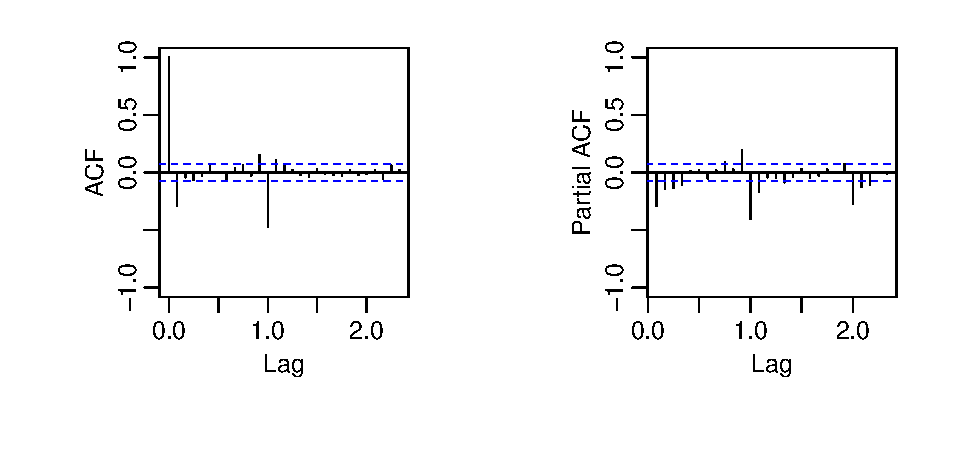
\includegraphics[width=\maxwidth]{figure/CO2-diff-1} 

\end{knitrout}
%%%%%%%%%%%%%%%%%%%%%%%%%%%
\end{center}
\caption{Correlogram and partial correlogram for the \CO\ data.}
\label{diff.fig}
\end{figure}

An STL decomposition of the series $\{x_t\}$, not plotted here, shows no remaining systematic trend and only tiny seasonal variation, strongly suggesting that the  differenced series is essentially stationary.

%%%%%%%%%%%%%%%%%%%%%%%%%%%

%%%%%%%%%%%%%%%%%%%%%%%%%%%

\section{Model-fitting}

We now\footnote{Following sections: description of the statistical model(s); application to the data; results and interpretation of the chosen model(s).}  try to fit to the data some seasonal ARIMA, $(p,d,q)\times(P,D,Q)_s$, models, using the usual notation; clearly for monthly data with an annual cycle, $s=12$.  In view of the trend and seasonality, and of the contents of Figure~\ref{diff.fig}, it seems best to try fitting low-order ARMA models to the series $x_t$ defined at (\ref{x.eqn}), so $d=D=1$.  Table~\ref{AIC.table} shows the maximised log likelihood and AIC values for the models up to orders $(1,1,1)\times (1,1,1)_{12}$. The increases in log likelihood and corresponding drops in AIC are largest when moving average components are added to the model.  The model with the smallest AIC among those fitted is $(1,1,1)\times (0,1,1)_{12}$, but three other ones are quite close: $(0,1,1)\times (1,1,1)_{12}$, $(1,1,1)\times (1,1,1)_{12}$, and the $(0,1,1)\times (0,1,1)_{12}$ that seemed indicated by the correlogram and partial correlogram. This last model and the best may be written as
\begin{eqnarray}
\label{fit011011.eqn}
x_t &=& (1-0.368_{0.042}B) (1-0.866_{0.022}B^{12})\varepsilon_t, \\
\label{fit111011.eqn}
x_t &=& 0.186_{0.107}X_{t-1}+(1-0.530_{0.093}B) (1-0.866_{0.022}B^{12})\varepsilon_t, 
\end{eqnarray}
with $\varepsilon_t \iid (0, 0.3^2)$ in both cases, where $B$ is the backshift operator and standard errors for coefficients appear as subscripts.  The AR(1) coefficient of the model (\ref{fit111011.eqn}) is not quite significant at the 95\% level, and including it strongly affects the MA(1) coefficient: in fact $-0.530+0.186=-0.344\approx -0.368$, so that the effect of adding the autoregressive term is to dilute the moving average term, because $(1+\alpha B)^{-1} \approx 1 - \alpha B$ for small $\alpha$. As AIC has a tendency to suggest overfitting, and as the likelihood ratio statistics for comparisons among these four models are barely significant, if at all, parsimony pushes us to favour the simplest of them, (\ref{fit011011.eqn}).  This has just two parameters, but the differencing that produced (\ref{x.eqn}) has removed a trend parameter and the month effects. Thus expression (\ref{fit011011.eqn}) implies that the corresponding model for the original data $y_t$ uses 15 parameters to explain the variation in 609 (correlated) observations; this seems a reasonable summary.

The interpretation of (\ref{fit011011.eqn}) in terms of the original data is complicated by the differencing. It is interesting, though perhaps a coincidence, that the variation in the data may be explained in terms of a moving average, which suggests that the \CO\  level at time $t$ is related to the quantity added to the atmosphere over the past year. This interpretation has to be tempered by the facts that the moving average model applies to the differenced data $X_t$ rather than to the original data, and that the moving average coefficients are negative, though this may be because of the differencing.

%%%%%%%%%%%%%%%%%%%%%%%%%%%

%%%%%%%%%%%%%%%%%%%%%%%%%%%

\begin{table}[ht!]
\begin{center}
\begin{tabular}{ccccccrr}
\toprule
$p$& $d$& $q$& $P$& $D$& $Q$& Log likelihood& AIC\\
\midrule
0&1&0&0&1&0&$-375.55$&$753.1$\\
1&1&0&0&1&0&$-345.18$&$694.36$\\
0&1&1&0&1&0&$-334.6$&$673.21$\\
0&1&0&1&1&0&$-288.07$&$580.13$\\
0&1&0&0&1&1&$-192.4$&$388.79$\\
1&1&0&1&1&0&$-256.29$&$518.59$\\
1&1&0&0&1&1&$-164.07$&$334.13$\\
0&1&1&1&1&0&$-245.34$&$496.68$\\
0&1&1&0&1&1&$-154.47$&$314.93$\\
1&1&1&1&1&0&$-242.48$&$492.96$\\
1&1&1&0&1&1&$-151.47$&$310.95$\\
0&1&1&1&1&1&$-154.46$&$316.93$\\
1&1&0&1&1&1&$-164.05$&$336.11$\\
1&1&1&1&1&1&$-151.47$&$312.95$\\
\bottomrule
\end{tabular}
\end{center}
\caption{Log likelihood and AIC values for  SARIMA $(p,d,q)\times(P,D,Q)_{12}$ models fitted to the \CO\  data.}
\label{AIC.table}
\end{table}

Plots of the usual time series diagnostics and of the cumulative periodogram, not shown here, confirm that the residuals from model (\ref{fit011011.eqn}) seem to be white noise, and a normal probability plot shows that the residuals are very close to normality.  

%%%%%%%%%%%%%%%%%%%%%%%%%%%

%%%%%%%%%%%%%%%%%%%%%%%%%%%

\section{Prediction}

In this section we discuss prediction of future ozone levels to the year 2020, based on the models fitted above.   One issue that often arises is that different almost equally plausible models may give rather different predictions, and then some sort of weighting may be required to produce an overall predictor taking this into account.  Often the weighting will be based on the relative plausibility of the different models, as judged by their relative likelihoods, analogous to Bayesian model averaging. Since the most plausible model in Table~\ref{AIC.table} has maximised log likelihood $\hat\ell$ of around $-131.78$, a model with $\hat\ell=-140$ would be roughly $\exp(140-132) \doteq e^8 = 2980$ times less likely than the best model, and it therefore seems reasonable to exclude models for which $\hat\ell<-140$. 

Figure~\ref{pred.fig} shows the data from the year 2001 onwards, with predictions and their 95\% confidence limits, for the six models in Table~\ref{AIC.table} for which the log likelihood exceeds $-140$. There is very little difference between them.  The level of 400ppmv is predicted to be breached for the first time in winter 2014--15, but the confidence intervals suggest that this might occur two years earlier, and by 2020 it seems very likely that the level will exceed 400ppmv throughout the year.  Closer inspection of the graphs suggests that these forecasts underestimate the rate of increase: the linear trend for the prediction period is below the average trend shown by the data over 1958--2008, because differencing to stabilise the series mean has not fully accounted for the slight convexity in the trend, which is therefore underestimated beyond the range of the data.  

The confidence bands shown in the figures account for the variability of the innovations, but not for model selection uncertainty or for the estimation uncertainty for the parameters.  Figure~\ref{pred.fig} suggests that model selection uncertainty is small, and as there are roughly 40 parameters for each observation, estimation uncertainty is small also.  The biggest source of prediction uncertainty is likely to be the failure of the model to match the trend immediately before the prediction period.  An attempt to account for this through a second differencing operation gave a worse fit, so within the SARIMA framework there seems to be little that can be done to remedy this.


\begin{figure}[p]
\begin{center}
%%%%%%%%%%%%%%%%%%%%%%%%%%%
\begin{knitrout}
\definecolor{shadecolor}{rgb}{0.969, 0.969, 0.969}\color{fgcolor}
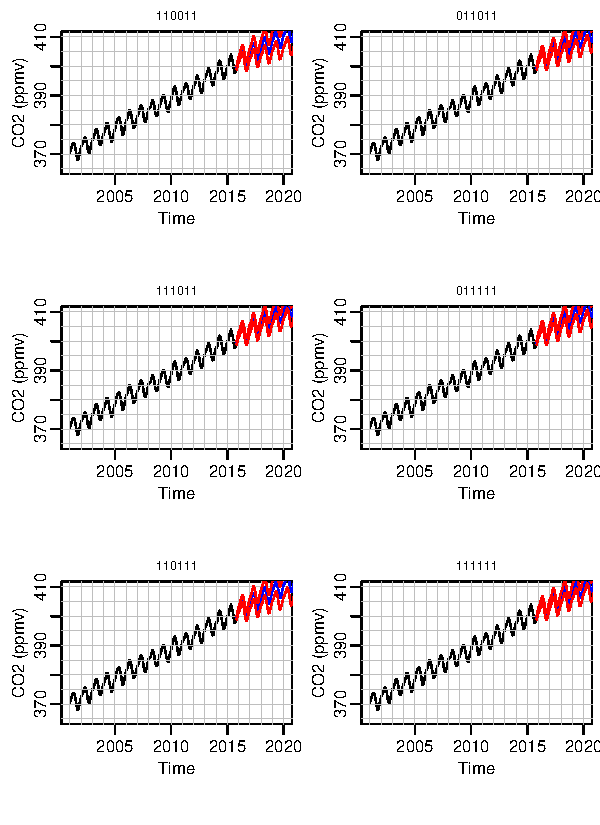
\includegraphics[width=\maxwidth]{figure/CO2-predict-1} 

\end{knitrout}
%%%%%%%%%%%%%%%%%%%%%%%%%%%
\end{center}
\caption{Comparison of predictions for levels of \CO\  (ppmv) for the period 2009--2020, for the six best models in Table~\ref{AIC.table}.  The data are shown in black, the predictions in blue, and 95\% pointwise prediction bands in red.  The grey grid is intended to aid comparison of the panels.}
\label{pred.fig}
\end{figure}



% Computations fitting SARIMA$(0,1,1)\times(0,1,1)_{12}$ model to data from 1990 onwards
% Predictions not used in report, but alluded to
%
% \begin{figure}[!f]
% \begin{center}
%' %%%%%%%%%%%%%%%%%%%%%%%%%%%%
%' <<begin.rcode, echo=FALSE, fig.width=6,fig.height=5>>=
%' fit011011 <- arima(window(co2,start=2000),order=c(0,1,1),seasonal=list(order=c(0,1,1),period=12))
%' pred <- predict(fit011011,133)
%' plot(window(co2,start=2001),ylim=c(365,410),xlim=c(2001,2020),main="011011",ylab="CO2 (ppmv)")
%' abline(h=hl,col="grey",lwd=lw)
%' abline(v=vl,col="grey",lwd=lw)
%' lines(pred$pred,col="blue")
%' lines(pred$pred+2*pred$se,col="red")
%' lines(pred$pred-2*pred$se,col="red")
%' @
%%%%%%%%%%%%%%%%%%%%%%%%%%%%
%\end{center}
%\caption{Predictions for levels of \CO\  (ppmv) for the period 2009--2020, for a SARIMA $(0,1,1)\times(01,1)_{12}$ model estimated from the data for 1990 onwards.}
%\label{predshort.fig}
%\end{figure}

\section{Discussion}

The\footnote{Final section: summary of the results; discussion of the advantages and  
limitations of the applied method; what else might be done, if time/data were available.} 
seasonal ARIMA model (\ref{fit011011.eqn}) seems to fit the data well, and its closest competitors among the SARIMA models fitted give very similar predictions, so one can have high confidence in them.  They are, however, compromised by the failure of the trends for the predictions to match the observed trend for the period immediately before 2008.  Fitting the SARIMA model from 1995 or 2000 onwards, not shown, does not seem to remedy this by giving a higher trend.  If more time were available, it would be worthwhile to investigate this more fully.  

A alternative and perhaps preferable approach would be to construct a suitable structural model \citep{Durbin.Koopman:2001}.

\bibliographystyle{CUP}
\bibliography{biblio}
	
\end{document}



